\documentclass[dsc,dvips]{coppe}
\usepackage[latin1]{inputenc}
\usepackage{amsmath,amssymb}

\makelosymbols
\makeloabbreviations

\begin{document}
  \title{Desenvolvimento de um Algoritmo Baseado no M�todo de Arnoldi para
  Solu��o de Problemas de Autovalor Generalizado}
  \foreigntitle{Solution of Generalized Eigensystems with Algorithms Based on
  Arnoldi Methods}
  \author{Camila}{Meyworm}
  \advisor{Prof.}{Carlos}{Magluta}{D.Sc.}
  \coadvisor{Prof.}{Fernando Luiz Bastos}{Ribeiro}{D.Sc.}
  \examiner{Prof.}{Alvaro Luiz Gayoso Azeredo Coutinho}{D.Sc.}
  \examiner{Prof.}{Webe Jo�o Mansur}{Ph.D.}
  \examiner{Prof.}{Paulo Batista Gon�alves}{D.Sc.}
  \department{PEMM}
  \date{12}{2008}
  \keyword{Problemas de Autovalor}
  \keyword{M�todo de Arnoldi}
  \keyword{An�lise Din�mica}
  \keyword{Palavra Chave}
  \maketitle

  \frontmatter
  \dedication{� minha m�e pelo dom da vida e pelo amparo ao longo desses anos.\\
�s minhas tias Vanete e Vanilde (\emph{in memoriam}).}


  \chapter*{Agradecimentos}

Agrade�o ao Conselho Nacional de Desenvolvimento Cient�fico e Tecnol�gico
(CNPq) pelo suporte financeiro.


  \begin{abstract}

Autovalores e autovetores de operadores lineares s�o importantes para muitas
�reas da Matem�tica Aplicada. Na Engenharia Civil, sobretudo na Engenharia de
Estruturas o uso de problemas de autovalor tem fundamental import�ncia, um
exemplo t�pico � a an�lise din�mica, onde os autovalores representam as
frequ�ncias naturais e os autovetores os modos de vibra��o associados � sua
frequ�ncia natural correspondente. A crescente demanda da avalia��o num�rica de
forma mais eficiente dessas quantidades, despertou o interesse na busca de
novos m�todos para a solu��o de problemas de autovalor, principalmente quando o
problema a ser analisado conduz a quantidades pertencentes ao conjunto dos
n�meros complexos.

\end{abstract}


  \begin{foreignabstract}

Eigenvalues and eigenvectors of linear operators are important in many Applied
Mathematics areas. In Civil Engineering, especially in Structural Analysis,
eigensystems have a fundamental importance. A typical example is in dynamic
analysis, where the eigenvalues represent the natural frequencies and
eigenvectors the mode shape. The increasing demand for efficient numeric
evaluation of eigenvalues and eigenvectors motivated the search for new methods
for the solution of complex eigensystems.

\end{foreignabstract}


  \tableofcontents
  \listoffigures
  \listoftables
  \printlosymbols
  \printloabbreviations

  \mainmatter
  \chapter{Introdu��o}

Em m�todos num�ricos para obter solu��es aproximadas de equa��es diferenciais,
tais como o m�todo dos elementos finitos (MEF)\abbrev{MEF}{m�todo de elementos
finitos} e o m�todo dos volumes finitos (MVF)\abbrev{MVF}{m�todo de volumes
finitos}, o dom�nio no qual estas equa��es foram definidas � discretizado em
sub-dom�nios simples denominados \textit{elementos}.

Denotemos o dom�nio por $\Omega$\symbl{$\Omega$}{dom�nio de defini��o de uma
equa��o diferencial}. Seja $\partial \Omega$ o contorno de
$\Omega$.\symbl{$\partial$}{operador do contorno.}

\section{Motiva�{\~ a}o}
adsadsda

\subsection{ASdasdsad}
adasda

\section{Objetivo}

\section{Metodologia}

\section{Organiza�{\~ a}o da tese}

  \chapter{Revis�o Bibliogr�fica}

No in�cio dos anos 50, LANCZOS~\cite{Lan50a} desenvolveu um m�todo para a
solu��o de problemas de autovalor sim�tricos, empregando transforma��es
similares, obtendo uma matriz da qual fosse mais simples obter seus autovalores
do que a matriz original do problema. ARNOLDI \cite{Arn51a} generalizou o
m�todo, estendendo-o para problemas n�o sim�tricos.


  \chapter{M�todo Proposto}

\section{O Algoritmo}

\begin{figure}[b]
\centering
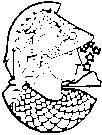
\includegraphics{minerva}
\caption{Deusa Minerva.}
\label{fig:minerva}
\end{figure}

  \chapter{Resultados e Discuss�es}

\section{Metodologia para avalia�{\~ a}o do M{\' e}todo}

\section{Valida�{\~ a}o da rotina implementada}

\subsection{Problema de autovalor padr{\~ a}o -- Caso I}

A Tabela~\ref{table:casoi} mostra as varia��es dos par�metros escolhidos para
an�lise.

\begin{table}[b]
\caption{Par{\^ a}metros do teste realizado com a matriz de Wilkinson,
3 autovalores computados.}
\label{table:casoi}
\centering
\begin{tabular}{cccc}
  \hline
  TValor de ``m'' & N$^{o}$ de itera�{\~ o}es & Tempo de CPU & Norma do Res{\' i}duo\\
  \hline
  6 & 100 & 0,09013 & $7,1474 \times 10^{-12}$\\
  10 & 28 & 0,09025 & $1,5387 \times 10^{-13}$\\
  20 & 10 & 0,100144 & $5,9011 \times 10^{-14}$\\
  40 & 6 & 0,16022 & $8,67438 \times 10^{-14}$\\
  50 & 3 & 0,24034 & $1,51537 \times 10^{-15}$\\
  \hline
\end{tabular}
\end{table}

  \chapter{Conclus�es}


  \backmatter
  \nocite{*}
  \bibliographystyle{coppe-unsrt}
  \bibliography{thesis}
  \appendix
  \chapter{C�digo Fonte}

\end{document}
